\documentclass[a4paper,11pt]{article}
\usepackage{amsmath,amsthm,amsfonts,amssymb,amscd,amstext,vmargin,graphics,graphicx,tabularx,multicol} 
\usepackage[francais]{babel}
\usepackage[utf8]{inputenc}  
\usepackage[T1]{fontenc} 
\usepackage{pstricks-add,tikz,tkz-tab,variations}
\usepackage[autolanguage,np]{numprint} 
\usepackage{xlop}


\setmarginsrb{1.5cm}{0.5cm}{1cm}{0.5cm}{0cm}{0cm}{0cm}{0cm} %Gauche, haut, droite, haut
\newcounter{numexo}
\newcommand{\exo}[1]{\stepcounter{numexo}\noindent{\bf \underline{Exercice~\thenumexo}}}
\reversemarginpar

\opset{decimalsepsymbol={,}}
\newcounter{enumtabi}
\newcounter{enumtaba}
\newcommand{\q}{\stepcounter{enumtabi} \theenumtabi.  }
\newcommand{\qa}{\stepcounter{enumtaba} (\alph{enumtaba}) }
\newcommand{\initq}{\setcounter{enumtabi}{0}}
\newcommand{\initqa}{\setcounter{enumtaba}{0}}

\newcommand\hole[1]{$\bullet$}

\newcommand{\be}{\begin{enumerate}}
\newcommand{\ee}{\end{enumerate}}
\newcommand{\bi}{\begin{itemize}}
\newcommand{\ei}{\end{itemize}}
\newcommand{\bp}{\begin{pspicture*}}
\newcommand{\ep}{\end{pspicture*}}
\newcommand{\bt}{\begin{tabular}}
\newcommand{\et}{\end{tabular}}
\renewcommand{\tabularxcolumn}[1]{>{\centering}m{#1}} %(colonne m{} centrée, au lieu de p par défault) 
\newcommand{\tnl}{\tabularnewline}

\newcommand{\bmul}[1]{\begin{multicols}{#1}}
\newcommand{\emul}{\end{multicols}}

\newcommand{\trait}{\noindent \rule{\linewidth}{0.2mm}}
\newcommand{\hs}[1]{\hspace{#1}}
\newcommand{\vs}[1]{\vspace{#1}}

\newcommand{\N}{\mathbb{N}}
\newcommand{\Z}{\mathbb{Z}}
\newcommand{\R}{\mathbb{R}}
\newcommand{\C}{\mathbb{C}}
\newcommand{\Dcal}{\mathcal{D}}
\newcommand{\Ccal}{\mathcal{C}}
\newcommand{\mc}{\mathcal}

\newcommand{\vect}[1]{\overrightarrow{#1}}
\newcommand{\ds}{\displaystyle}
\newcommand{\eq}{\quad \Leftrightarrow \quad}
\newcommand{\vecti}{\vec{\imath}}
\newcommand{\vectj}{\vec{\jmath}}
\newcommand{\Oij}{(O;\vec{\imath}, \vec{\jmath})}
\newcommand{\OIJ}{(O;I,J)}




\newcommand{\reponse}[1][1]{%
\multido{}{#1}{\makebox[\linewidth]{\rule[0pt]{0pt}{20pt}\dotfill}
}}

\newcommand{\titre}[5] 
% #1: titre #2: haut gauche #3: bas gauche #4: haut droite #5: bas droite
{
\noindent #2 \hfill #4 \\
#3 \hfill #5

\vspace{-1.6cm}

\begin{center}\rule{6cm}{0.5mm}\end{center}
\vspace{0.2cm}
\begin{center}{\large{\textbf{#1}}}\end{center}
\begin{center}\rule{6cm}{0.5mm}\end{center}
}



\begin{document}
\pagestyle{empty}
\titre{Chapitre 2 : Les nombres décimaux}{}{}{}{}

\vspace*{1cm}

\begin{center}
{\Large \textbf{Niveau 1 :}}
\end{center}

\vspace*{1cm}

$\rightarrow$ \textbf{Vocabulaire de la multiplication}\\


\exo \\ Écrire une phrase pour traduire chacune des égalités avec les mots : \textit{produit} et \textit{facteur}.\\

\initqa
\qa 41,7 $\times$ 6,8 = 638,56\\
Le . . . . . . . . . . des . . . . . . . . . 41,7 et 6,8 vaut 638,56.\\

\qa 14 $\times$ 32,4 = 453,6\\
Le . . . . . . . . . . des . . . . . . . . . 14 et 32,4 vaut 453,6.\\


\exo \\ Traduire les expressions suivantes par un calcul.\\

\initqa \qa Le produit de 4 par 8 : . . . . . . . . . . . . . . . . . . . . . .\\

\qa La somme de 5 et de 19 : . . . . . . . . . . . . . . . . . . . . . .\\

\qa La différence de 201 et de 56 : . . . . . . . . . . . . . . . . . . . . . .\\





\vspace*{0.5cm}

$\rightarrow$ \textbf{Multiplication posée}\\

\exo \\ Effectuer les opérations suivantes.\\

\opmul[carryadd=false,resultstyle=\white]{167}{8} \hspace*{2cm} \opmul[carryadd=false,resultstyle=\white]{1 253}{6}\\

\exo \\ Effectuer les opérations suivantes.\\

\opmul[carryadd=false,resultstyle=\white]{219}{5} \hspace*{2cm} \opmul[carryadd=false,resultstyle=\white]{31 695}{8}\\

\exo \\ Effectuer les opérations suivantes.\\

\opmul[carryadd=false,resultstyle=\white]{317}{6} \hspace*{2cm} \opmul[carryadd=false,resultstyle=\white]{52 784}{7}\\


\vspace*{0.5cm}

$\rightarrow$ \textbf{Calculs en ligne :astucieux, $\times$ 10 ..., $\times$ 0,1 ..., placement virgule) }\\

\exo \\ Calculer les produits suivants en effectuant des regroupements astucieux.\\

\initqa \qa  5 $\times$ 63,5  $\times$ 2 = . . . . . . .\\

\qa  50 $\times$ 8  $\times$ 2 $\times$ 7 = . . . . . . .\\

\qa 20 $\times$ 1,25  $\times$ 5 = . . . . . . .\\


\exo \\ Calculer les produits suivants en effectuant des regroupements astucieux.\\

\initqa \qa  5 $\times$ 75 $\times$ 5  $\times$ 4 = . . . . . . .\\

\qa  5 $\times$ 6 $\times$ 7 $\times$ 2 = . . . . . . .\\

\qa 2 $\times$ 24,5  $\times$ 50 = . . . . . . .\\


\exo \\ Calculer les produits suivants.\\

\initqa \qa 23 $\times$ 100 = . . . .\\

\qa 10 $\times$ 51 = . . . .\\

\qa 146 $\times$ 10 = . . . .\\

\qa 934 $\times$ 100 = . . . .\\


\exo \\ Calculer les produits suivants.\\

\initqa \qa 62 $\times$ 0,1 = . . . .\\

\qa 783 $\times$ 0,1 = . . . .\\

\qa 1 492 $\times$ 0,1 = . . . .\\

\qa 560 $\times$ 0,1 = . . . .\\



\exo \\ Compléter par 10 ; 100 ; ... ; 0,1 ; 0,01 ; ... ou le nombre qui convient.\\

\initqa \qa 320 $\times$  . . . . = 3 200\\

\qa 12,1 $\times$  . . . . = 1,21\\

\qa . . . . $\times$  0,1 = 74,3\\

\qa . . . . $\times$ 10 = 8,6\\

\exo \\ Pour chacun des calculs suivants, réécrire le résultat en plaçant une virgule au bon endroit pour qu'il soit correct.\\

\initqa \qa 2,7 $\times$ 17,5 = 4725\\

\qa 12,75 $\times$ 9 = 11475\\


\qa 0,55 $\times$ 12,5 = 6875\\


\qa 25,75 $\times$ 0,8 = 20600\\



\vspace*{0.5cm}

$\rightarrow$ \textbf{Calcul mental (Tale de multiplication, Ordre de grandeur) }\\

\exo \\ Choisir le meilleur ordre de grandeur de chaque produit.\\

\begin{tabular}{|c|c|c|c|}
\hline 
Calculs & \multicolumn{3}{c|}{Ordre de grandeur du produit} \\ 
\hline 
25,3 $\times$ 6 & 150 & 170 & 180 \\ 
\hline 
18,7 $\times$ 4,2 & 40 & 80 & 100 \\ 
\hline 
247 $\times$ 5 & 1 000 & 1 250 & 1 500 \\ 
\hline 
\end{tabular} 


\exo \\ Compléter les égalités suivantes.\\

\initqa \qa 2 $\times$ 7 = . . . \\

\qa 3 $\times$ 8 = . . . \\

\qa 4 $\times$ 7 = . . . \\

\qa 6 $\times$ 9 = . . . \\

\qa 7 $\times$ 7 = . . . \\

\qa 8 $\times$ 6 = . . . \\


\exo \\ Dans chaque cas, retrouver le nombre manquant.\\

\initqa \qa 9 $\times$ . . .  = 9 \\

 \qa 8 $\times$ . . .  = 0 \\
 
  \qa 3 $\times$ . . .  = 18 \\
  
   \qa 6 $\times$ . . .  = 42 \\
   
   
   \exo \\ Compléter la table de multiplication suivante.\\
   
   \begin{tabular}{|c|c|c|c|}
   \hline 
   $\times$ & 5 & 6 & 7 \\ 
   \hline 
   2 & . . . & . . . & . . . \\ 
   \hline 
   3 & . . . & . . . & . . . \\ 
   \hline 
   4 & . . . & . . . & . . . \\ 
   \hline 
   \end{tabular} 


\vspace*{0.5cm}





$\rightarrow$ \textbf{Problèmes en lien avec la multiplication }\\



\exo \\ Dans un immeuble de 6 étages, il y a 8 appartements par étage.\\
Combien y a-t-il d'appartements dans cet immeuble ?\\

Calculs en ligne : \\
\reponse[2]\\


Phrase réponse :\\
L'immeuble possède . . . appartements.\\


\exo \\ Un jour de canicule. Marius a bu 3 bouteilles d'eau de 1,5 L chacune.\\
Quelle quantité d'eau a-t-il bue ?\\

Calculs en ligne : \\
\reponse[2]\\


Phrase réponse :\\
Marius a bu . . . L d'eau.\\



\exo \\ Une sauterelle fait des bonds de 5,4 m.\\
Quelle distance parcourt-elle en 11 bonds ?\\


Calculs en ligne : \\
\reponse[2]\\


Phrase réponse :\\
La sauterelle a parcouru . . . m en 11 bonds.\\







\vspace*{0.5cm}
\begin{center}
{\Large \textbf{Niveau 2 :}}
\end{center}

\vspace*{1cm}

$\rightarrow$ \textbf{Vocabulaire de la multiplication}\\


\exo \\ Écrire une phrase pour traduire chacune des égalités avec les mots : \textit{produit} et \textit{facteur}.\\

\initqa
\qa 254,1 $\times$ 2,4 = 609,84\\
\reponse[1]\\

\qa 52,31 $\times$ 108,6 = 5 680,866\\
\reponse[1]\\


\exo \\ Traduire les expressions suivantes par un calcul.\\

\initqa \qa Le produit de 7,1 par 6,5 : . . . . . . . . . . . . . . . . . . . . . .\\

\qa La somme de 36,15 et de 7,09 : . . . . . . . . . . . . . . . . . . . . . .\\

\qa La somme de 8 et du produit de 3 par 5 : . . . . . . . . . . . . . . . . . . . . . .\\


\vspace*{0.5cm}

$\rightarrow$ \textbf{Multiplication posée}\\

\exo \\ Effectuer les opérations suivantes.\\

\opmul[carryadd=false,displayintermediary=None,resultstyle=\white]{67}{14} \hspace*{2cm} \opmul[carryadd=false,displayintermediary=None,resultstyle=\white]{13025}{78}\\

\exo \\ Effectuer les opérations suivantes.\\

\opmul[carryadd=false,displayintermediary=None,resultstyle=\white]{78}{36} \hspace*{2cm} \opmul[carryadd=false,displayintermediary=None,resultstyle=\white]{61207}{25}\\

\exo \\ Effectuer les opérations suivantes.\\

\opmul[carryadd=false,displayintermediary=None,resultstyle=\white]{85}{29} \hspace*{2cm} \opmul[carryadd=false,displayintermediary=None,resultstyle=\white]{70158}{46}\\






$\rightarrow$ \textbf{Calculs en ligne :astucieux, $\times$ 10 ..., $\times$ 0,1 ..., placement virgule) }\\

\exo \\ Calculer les produits suivants en effectuant des regroupements astucieux.\\

\initqa \qa  25 $\times$ 8  $\times$ 4 $\times$ 5  = . . . . . . .\\

\qa  2 500 $\times$ 3,8  $\times$ 4 $\times$ 2 = . . . . . . .\\

\qa 5 000 $\times$ 17  $\times$ 19 $\times$ 0 $\times$ 180 $\times$ 4 = . . . . . . .\\


\exo \\ Calculer les produits suivants en effectuant des regroupements astucieux.\\

\initqa \qa  2 $\times$ 136,2 $\times$ 500  = . . . . . . .\\

\qa  0,8 $\times$ 2 $\times$ 0,6 $\times$ 50 = . . . . . . .\\

\qa 2,18 $\times$ 0,001  $\times$ 1 000 = . . . . . . .\\


\exo \\ Calculer les produits suivants.\\

\initqa \qa 5,378 $\times$ 100 = . . . .\\

\qa 71,47 $\times$ 100 = . . . .\\

\qa 0,58 $\times$ 10 = . . . .\\

\qa 6,3 $\times$ 10 = . . . .\\


\exo \\ Calculer les produits suivants.\\

\initqa \qa 120 $\times$ 0,1 = . . . .\\

\qa 1,5 $\times$ 0,1 = . . . .\\

\qa 11,2 $\times$ 0,1 = . . . .\\

\qa 10 $\times$ 0,1 = . . . .\\



\exo \\ Compléter par 10 ; 100 ; ... ; 0,1 ; 0,01 ; ... ou le nombre qui convient.\\

\initqa \qa 21 $\times$  . . . . = 2 100\\

\qa 5,13 $\times$  . . . . = 0,513\\

\qa . . . . $\times$  100 = 510\\

\qa 12,4 $\times$ . . . . = 0,124\\

\exo \\ Pour chacun des calculs suivants, réécrire le résultat en plaçant une virgule au bon endroit pour qu'il soit correct. (en ajoutant éventuellement des zéros.)\\

\initqa \qa 12,8 $\times$ 5,3 = 6784\\

\qa 28,7 $\times$ 1,04 = 29848\\


\qa 0,15 $\times$ 6,3 = 945\\


\qa 0,008 $\times$ 543,9 = 43512\\






$\rightarrow$ \textbf{Calcul mental (Tale de multiplication, Ordre de grandeur) }\\

\exo \\ Choisir le meilleur ordre de grandeur de chaque produit.\\

\begin{tabular}{|c|c|c|c|}
\hline 
Calculs & \multicolumn{3}{c|}{Ordre de grandeur du produit} \\ 
\hline 
2 $\times$ 4 867 & 10 000 & 8 000 & 6 000 \\ 
\hline 
24 $\times$ 10,5 & 240 & 2 400 & 34 \\ 
\hline 
30,21 $\times$ 7,4 & 210 & 225 & 240 \\ 
\hline 
\end{tabular} 


\exo \\ Compléter les égalités suivantes.\\

\initqa \qa 9 $\times$ 7 = . . . \\

\qa 6 $\times$ 8 = . . . \\

\qa 3 $\times$ 8 = . . . \\

\qa 8 $\times$ 9 = . . . \\

\qa 9 $\times$ 5 = . . . \\

\qa 7 $\times$ 6 = . . . \\


\exo \\ Dans chaque cas, retrouver le nombre manquant.\\

\initqa \qa 6 $\times$ . . .  = 24 \\

 \qa 7 $\times$ . . .  = 63 \\
 
  \qa 18 = 6 $\times$ . . .  \\
  
   \qa 24 = 8 $\times$ . . .  \\
   
   
   \exo \\ Compléter la table de multiplication suivante.\\
   
   \begin{tabular}{|c|c|c|c|}
   \hline 
   $\times$ & 6 & 8 & 9 \\ 
   \hline 
   4 & . . . & . . . & . . . \\ 
   \hline 
   6 & . . . & . . . & . . . \\ 
   \hline 
   7 & . . . & . . . & . . . \\ 
   \hline 
   \end{tabular} 

$\rightarrow$ \textbf{Problèmes en lien avec la multiplication }\\



\exo \\ Pour un stage de voile, on constitue 6 groupes de 7 personnes et 9 groupes de 8 personnes.\\
Combien y a-t-il de participants ?\\

Calculs en ligne : \\
\reponse[2]\\


Phrase réponse :\\
\reponse[1]\\

\exo \\ Pour un stage de voile, on constitue 6 groupes de 7 personnes et 9 groupes de 8 personnes.\\
Combien y a-t-il de participants ?\\

Calculs en ligne : \\
\reponse[2]\\


Phrase réponse :\\
\reponse[1]\\


\exo \\ Lou achète 4 kg d'oranges à 3,60 euros le kilogramme.\\
Combien va-t-elle payer ?\\

Calculs en ligne : \\
\reponse[2]\\


Phrase réponse :\\
\reponse[1]\\



\exo \\ Un pâtissier a utiliser 15 boîtes de 12 oeufs et une boîte de 6 oeufs.\\
Combien a-t-il utilisé d'oeufs en tout ?\\

Calculs en ligne : \\
\reponse[2]\\


Phrase réponse :\\
\reponse[1]\\

\begin{center}
{\Large \textbf{Niveau 3 :}}
\end{center}

\vspace*{1cm}

$\rightarrow$ \textbf{Vocabulaire de la multiplication}\\





\exo \\ Écrire le calcul correspondant à chaque phrase.\\

\initqa \qa La somme de 30 et du produit de 2 par 12 : . . . . . . . . . . . . . . . . . . . . . .\\

\qa Le produit des 3 nombres 2 ; 5 et 7 : . . . . . . . . . . . . . . . . . . . . . .\\

\qa Le produit de 15 par le double de 5,5  : . . . . . . . . . . . . . . . . . . . . . .\\


\exo \\ Traduire chaque expression par une phrase.\\

\initqa
\qa 9,1 $\times$ 14\\
\reponse[1]\\

\qa 5 $\times$ (7 - 3)\\
\reponse[1]\\


\vspace*{0.5cm}

$\rightarrow$ \textbf{Multiplication posée}\\

\exo \\ Effectuer les opérations suivantes.\\

\opmul[carryadd=false,displayintermediary=None,resultstyle=\white]{52}{1.8} \hspace*{2cm} \opmul[carryadd=false,displayintermediary=None,resultstyle=\white]{1,3}{5.7}\\

\exo \\ Effectuer les opérations suivantes.\\

\opmul[carryadd=false,displayintermediary=None,resultstyle=\white]{93.76}{6} \hspace*{2cm} \opmul[carryadd=false,displayintermediary=None,resultstyle=\white]{10.2}{35.1}\\

\exo \\ Effectuer les opérations suivantes.\\

\opmul[carryadd=false,displayintermediary=None,resultstyle=\white]{0.28}{7} \hspace*{2cm} \opmul[carryadd=false,displayintermediary=None,resultstyle=\white]{5.97}{6.2}\\

\exo \\ Compléter la multiplication suivante.\\

\opmul[carryadd=false,displayintermediary=None,operandstyle.2.1=\hole,resultstyle.1=\hole]{934}{7}\\




$\rightarrow$ \textbf{Calculs en ligne :astucieux, $\times$ 10 ..., $\times$ 0,1 ..., placement virgule) }\\

\exo \\ Calculer les produits suivants en effectuant des regroupements astucieux.\\

\initqa \qa  0,25 $\times$ 9  $\times$ 4 $\times$ 8  = . . . . . . .\\

\qa  0,1 $\times$ 14  $\times$ 1 000 = . . . . . . .\\

\qa 0,25 $\times$ 12,38  $\times$ 4 = . . . . . . .\\


\exo \\ Calculer les produits suivants en effectuant des regroupements astucieux.\\

\initqa \qa  0,9 $\times$ 2 $\times$ 0,7 $\times$ 50  = . . . . . . .\\

\qa  2,5 $\times$ 3 $\times$ 4 $\times$ 9 = . . . . . . .\\

\qa 5 000 $\times$ 7,6  $\times$ 0,02 = . . . . . . .\\


\exo \\ Calculer les produits suivants.\\

\initqa \qa 0,7 $\times$ 100 = . . . .\\

\qa 3,57 $\times$ 1 000 = . . . .\\

\qa 72,6 $\times$ 100 = . . . .\\

\qa 0,057 $\times$ 10 = . . . .\\


\exo \\ Calculer les produits suivants.\\

\initqa \qa 2 000 $\times$ 0,01 = . . . .\\

\qa 352 $\times$ 0,01 = . . . .\\

\qa 100 $\times$ 0,01 = . . . .\\

\qa 0,87 $\times$ 0,01 = . . . .\\



\exo \\ Compléter par 10 ; 100 ; ... ; 0,1 ; 0,01 ; ... ou le nombre qui convient.\\

\initqa \qa 8,79 $\times$  . . . . = 87,9\\

\qa 480 $\times$  . . . . = 4,8\\

\qa . . . . $\times$  0,1 = 0,017\\

\qa 0,028 $\times$ . . . . = 2,8\\

\exo \\ Pour chacun des calculs suivants, réécrire le résultat en plaçant une virgule au bon endroit pour qu'il soit correct. (en ajoutant éventuellement des zéros.)\\

\initqa \qa 12,7 $\times$ 2,4 = 3048\\

\qa 0,14 $\times$ 5,9 = 826\\


\qa 0,007 $\times$ 573,2 = 40124\\


\qa 0,245 $\times$ 0,125 = 30625\\


$\rightarrow$ \textbf{Calcul mental (Tale de multiplication, Ordre de grandeur) }\\

\exo \\ Choisir le meilleur ordre de grandeur de chaque produit.\\

\begin{tabular}{|c|c|c|c|}
\hline 
Calculs & \multicolumn{3}{c|}{Ordre de grandeur du produit} \\ 
\hline 
84 $\times$ 1,05 & 1 000 & 10 & 100 \\ 
\hline 
9,8 $\times$ 6,07 & 54 & 60 & 70 \\ 
\hline 
75 $\times$ 0,39 & 30 & 37,5 & 70 \\ 
\hline 
\end{tabular} 


\exo \\ Compléter les égalités suivantes.\\

\initqa \qa 9 $\times$ 11 = . . . \\

\qa 10 $\times$ 12 = . . . \\

\qa 8 $\times$ 7 = . . . \\

\qa 13 $\times$ 3 = . . . \\

\qa 15 $\times$ 4 = . . . \\

\qa 0,2 $\times$ 5 = . . . \\


\exo \\ Dans chaque cas, retrouver le nombre manquant.\\

\initqa \qa 4 $\times$ . . . $\times$ 2  = 56 \\

 \qa 5 $\times$ . . . $\times$ . . .   = 30 \\
 
  \qa 7 $\times$ . . . = 77 \\
  
   \qa 48 = 4 $\times$ . . .  \\
   
   
   \exo \\ Compléter la table de multiplication suivante.\\
   
   \begin{tabular}{|c|c|c|c|}
   \hline 
   $\times$ & 9 & 7 & 8 \\ 
   \hline 
   3 & . . . & . . . & . . . \\ 
   \hline 
   8 & . . . & . . . & . . . \\ 
   \hline 
   9 & . . . & . . . & . . . \\ 
   \hline 
   \end{tabular}


$\rightarrow$ \textbf{Problèmes en lien avec la multiplication }\\



\exo \\ Pour une sortie scolaire les professeurs prévoient 128 de ces paquets de biscuits.\\
Calculer le prix total des biscuits à payer.\\


\includegraphics[scale=1]{pbmul1.eps} \\

Calculs en ligne : \\
\reponse[2]\\


Phrase réponse :\\
\reponse[1]\\


\exo \\ 1 kg de poisson coûte 23,70 euros.\\
Quel est le prix de 6,8 kg de ce poisson ?\\

Calculs en ligne : \\
\reponse[2]\\


Phrase réponse :\\
\reponse[1]\\

\exo \\ On se propose de calculer le prix à payer pour l'achat du jambon ci-dessous.\\

\includegraphics[scale=0.4]{pbmul2.eps} \\

Calculs en ligne : \\
\reponse[2]\\


Phrase réponse :\\
\reponse[1]\\

\exo \\ Un kilogramme de rôti coûte 15,25 euros.\\
Combien coûte un rôti pesant 3,2 kg ?\\

Calculs en ligne : \\
\reponse[2]\\


Phrase réponse :\\
\reponse[1]\\



\begin{center}
{\Large \textbf{Niveau 4:}}
\end{center}

\vspace*{1cm}

$\rightarrow$ \textbf{Vocabulaire de la multiplication}\\





\exo \\ Écrire le calcul correspondant à chaque phrase.\\

\initqa \qa La différence entre 28 et le produit de 3 par 7 : . . . . . . . . . . . . . . . . . . . . . .\\

\qa Le produit de 5 par la somme de 7 et de 2 : . . . . . . . . . . . . . . . . . . . . . .\\

\qa Le produit de la différence de 17 et 4 par 2  : . . . . . . . . . . . . . . . . . . . . . .\\


\exo \\ Traduire chaque expression par une phrase.\\

\initqa
\qa 109,5 - 7,43\\
\reponse[1]\\

\qa (15 + 13) $\times$ 3\\
\reponse[1]\\


$\rightarrow$ \textbf{Multiplication posée}\\

\exo \\ Effectuer les opérations suivantes.\\

\opmul[carryadd=false,displayintermediary=None,resultstyle=\white]{63}{0.7} \hspace*{2cm} \opmul[carryadd=false,displayintermediary=None,resultstyle=\white]{4.38}{5.7}\\

\exo \\ Effectuer les opérations suivantes.\\

\opmul[carryadd=false,displayintermediary=None,resultstyle=\white]{356.1}{9.4} \hspace*{2cm} \opmul[carryadd=false,displayintermediary=None,resultstyle=\white]{2.08}{4.67}\\

\exo \\ Effectuer les opérations suivantes.\\

\opmul[carryadd=false,displayintermediary=None,resultstyle=\white]{6.93}{15.81} \hspace*{2cm} \opmul[carryadd=false,displayintermediary=None,resultstyle=\white]{14.95}{0.67}\\

\exo \\ Compléter la multiplication suivante.\\

\opmul[carryadd=false,displayintermediary=None,operandstyle.1.1=\hole,operandstyle.1.2=\hole,operandstyle.1.3=\hole]{525}{7}\\


\exo \\ Compléter la multiplication suivante.\\

\opmul[carryadd=false,displayintermediary=None,operandstyle.1.3=\hole,operandstyle.2.1=\hole,resultstyle.1=\hole]{2023}{6}\\


$\rightarrow$ \textbf{Calculs en ligne :astucieux, $\times$ 10 ..., $\times$ 0,1 ..., placement virgule) }\\

\exo \\ Calculer les produits suivants en effectuant des regroupements astucieux.\\

\initqa \qa  4 $\times$ 3,9  $\times$ 0,25  = . . . . . . .\\

\qa  8 $\times$ 52  $\times$ 12,5 = . . . . . . .\\

\qa 32 $\times$ 0,2  $\times$ 5 $\times$ 3 = . . . . . . .\\


\exo \\ Calculer les produits suivants en effectuant des regroupements astucieux.\\

\initqa \qa  0,75 $\times$ 0,06 $\times$ 4   = . . . . . . .\\

\qa  8 $\times$ 49 $\times$ 1,25  = . . . . . . .\\

\qa 2,5 $\times$ 1,7  $\times$ 0,4 = . . . . . . .\\


\exo \\ Calculer les produits suivants.\\

\initqa \qa 0,065 $\times$ 10 = . . . .\\

\qa 11,11 $\times$ 1 000 = . . . .\\

\qa 0,9 $\times$ 100 = . . . .\\

\qa 27,3 $\times$ 10 000 = . . . .\\


\exo \\ Calculer les produits suivants.\\

\initqa \qa 463 $\times$ 0,001 = . . . .\\

\qa 1 257 $\times$ 0,001 = . . . .\\

\qa 1 000 $\times$ 0,001 = . . . .\\

\qa 37,1 $\times$ 0,001 = . . . .\\



\exo \\ Compléter par 10 ; 100 ; ... ; 0,1 ; 0,01 ; ... ou le nombre qui convient.\\

\initqa \qa 0,32 $\times$  . . . . = 320\\

\qa . . . .  $\times$  27 = 0,027\\

\qa . . . . $\times$  0,01 = 1,57\\

\qa 5,926 $\times$ . . . . = 592,6\\

\exo \\ Pour chacun des calculs suivants, réécrire le nombre souligné en plaçant une virgule au bon endroit pour que l'égalité soit vraie.\\

\initqa \qa 3,42 $\times$ \underline{271} = 9,268 2\\

\qa \underline{432} $\times$ 0,614 = 26,524 8\\


\qa 0,48 $\times$ \underline{62} = 29,76\\


\qa 2,6 $\times$ \underline{485} = 126,1\\



$\rightarrow$ \textbf{Calcul mental (Tale de multiplication, Ordre de grandeur) }\\

\exo \\ Choisir le meilleur ordre de grandeur de chaque produit.\\

\begin{tabular}{|c|c|c|c|}
\hline 
Calculs & \multicolumn{3}{c|}{Ordre de grandeur du produit} \\ 
\hline 
31 $\times$ 6 015 & 18 000 & 180 000 & 1 800 000 \\ 
\hline 
57,83 $\times$ 28,79 & 18 & 180 & 1 800 \\ 
\hline 
38,45 $\times$ 19,87 & 700 & 800 & 900 \\ 
\hline 
\end{tabular} 


\exo \\ Compléter les égalités suivantes.\\

\initqa \qa 0,5 $\times$ 14= . . . \\

\qa 14 $\times$ 7 = . . . \\

\qa 1,21 $\times$ 2 = . . . \\

\qa 0,7 $\times$ 3 = . . . \\

\qa 0,4 $\times$ 25 = . . . \\

\qa 0,41 $\times$ 4 = . . . \\


\exo \\ Dans chaque cas, retrouver le nombre manquant.\\

\initqa \qa 7 $\times$ . . .  = 560 \\

 \qa . . . $\times$ 2 $\times$ 3   = 54 \\
 
  \qa 6 $\times$ . . . = 3 600 \\
  
   \qa 51 = 102 $\times$ . . .  \\
   
   
   \exo \\ Compléter la table de multiplication suivante.\\
   
   \begin{tabular}{|c|c|c|c|}
   \hline 
   $\times$ & . . . & . . . & 6 \\ 
   \hline 
  7 & 21 & . . . & . . . \\ 
   \hline 
  8 & . . . & 64 & . . . \\ 
   \hline 
  4 & . . . & . . . & . . . \\ 
   \hline 
   \end{tabular}
   
   
   $\rightarrow$ \textbf{Problèmes en lien avec la multiplication }\\



\exo \\ Une salle de spectacle contient 42 rangées dont 17 rangées de 30 sièges. Les autres ont 24 sièges.\\
Calculer le nombre total de sièges dans cette salle.\\

Calculs en ligne : \\
\reponse[2]\\


Phrase réponse :\\
\reponse[1]\\


\exo \\ Un camion transporte 100 palettes. Chaque palette contient 10 packs de 6 bouteilles d'eau minéral de 1,5 L chacune.\\
Combien de litres d'eau transporte ce camion ?\\

Calculs en ligne : \\
\reponse[2]\\


Phrase réponse :\\
\reponse[1]\\

\exo \\ Passer une annonce dans un journal coûte 23,59 euros, puis il faut rajouter 8,50 euros par ligne.\\
Quel est le prix de l'annonce ci-dessous ?\\


\includegraphics[scale=1]{pbmul3.eps} \\

Calculs en ligne : \\
\reponse[2]\\


Phrase réponse :\\
\reponse[1]\\

   
\begin{center}
{\Large \textbf{Niveau 5 :}}
\end{center}

\vspace*{1cm}

$\rightarrow$ \textbf{Vocabulaire de la multiplication}\\





\exo \\ 

\initq \q Quel est :\\
\initqa \qa le double de 14,8 ? . . . . . . . .\\
\qa le triple de 5,4 ? . . . . . . . . . .\\
\qa le quadruple de 6,3 ? . . . . . . . . . . .\\

\q Combien vaut le produit du double de 7 par le triple de 5 ? . . . . .\\

\exo \\ Traduire chaque expression par une phrase.\\

\initqa
\qa (7 - 2) $\times$ 4 \\
\reponse[1]\\

\qa (19 + 7) $\times$ (1 + 8)\\
\reponse[1]\\

\exo \\ Traduire chaque expression par une phrase.\\

\initqa
\qa 8 $\times$ (10 - 5) \\
\reponse[1]\\

\qa (7 - 4) $\times$ (10 + 18)\\
\reponse[1]\\

$\rightarrow$ \textbf{Multiplication posée}\\

\exo \\ Effectuer les opérations suivantes.\\

\opmul[carryadd=false,displayintermediary=None,resultstyle=\white]{1.7}{0.09} \hspace*{2cm} \opmul[carryadd=false,displayintermediary=None,resultstyle=\white]{8.35}{0.16}\\

\exo \\ Effectuer les opérations suivantes.\\

\opmul[carryadd=false,displayintermediary=None,resultstyle=\white]{0.17}{0.58} \hspace*{2cm} \opmul[carryadd=false,displayintermediary=None,resultstyle=\white]{0.43}{5.09}\\



\exo \\ Compléter la multiplication suivante.\\

\opmul[carryadd=false,operandstyle.1.1=\hole,intermediarystyle.1.1=\hole,intermediarystyle.1.3=\hole,intermediarystyle.2.1=\hole,intermediarystyle.2.3=\hole,operandstyle.2.1=\hole,operandstyle.2.2=\hole]{27}{76}\\


\exo \\ Compléter la multiplication suivante.\\

\opmul[carryadd=false,operandstyle.1.2=\hole,operandstyle.2.1=\hole,intermediarystyle.2.1=\hole,intermediarystyle.2.1=\hole,intermediarystyle.2.3=\hole,resultstyle=\hole]{158}{34}\\


\exo \\ Compléter la multiplication suivante.\\

\opmul[carryadd=false,operandstyle.1.1=\hole,operandstyle.1.2=\hole,intermediarystyle.1.3=\hole,intermediarystyle.2.3=\hole,intermediarystyle.2.4=\hole,resultstyle=\hole]{321}{43}\\


\exo \\ Compléter la multiplication suivante.\\

\opmul[carryadd=false,operandstyle.2.1=\hole,operandstyle.2.2=\hole,intermediarystyle.1.1=\hole,intermediarystyle.1.2=\hole,intermediarystyle.1.3=\hole,intermediarystyle.1.4=\hole,resultstyle.3=\hole,resultstyle.4=\hole,resultstyle.5=\hole]{702}{74}\\

\exo \\ Compléter la multiplication suivante.\\

\opmul[carryadd=false,operandstyle.1.2=\hole,operandstyle.1.3=\hole,operandstyle.2.1=\hole,operandstyle.2.2=\hole,intermediarystyle.1.6=\hole,intermediarystyle.2.2=\hole,intermediarystyle.2.3=\hole,intermediarystyle.2.4=\hole,intermediarystyle.2.5=\hole,intermediarystyle.2.6=\hole,resultstyle=\hole]{37037}{18}\\



$\rightarrow$ \textbf{Calculs en ligne :astucieux, $\times$ 10 ..., $\times$ 0,1 ..., placement virgule) }\\

\exo \\ Calculer les produits suivants en effectuant des regroupements astucieux.\\

\initqa \qa  0,2 $\times$ 1,2  $\times$ 0,5 $\times$ 7  = . . . . . . .\\

\qa  0,4 $\times$ 5,6  $\times$ 25 $\times$ 0,2 = . . . . . . .\\

\qa 5 $\times$ 1,7  $\times$ 0,4  $\times$ 20 = . . . . . . .\\


\exo \\ Calculer les produits suivants en effectuant des regroupements astucieux.\\

\initqa \qa  0,25 $\times$ 0,5 $\times$ 3,7 $\times$ 4 $\times$ 2  = . . . . . . .\\

\qa  32 $\times$ 0,5 $\times$ 0,2 $\times$ 3 = . . . . . . .\\

\qa 1,2 $\times$ 0,25  $\times$ 40 $\times$ 5 = . . . . . . .\\


\exo \\ Calculer les produits suivants.\\

\initqa \qa 0,4 $\times$ 1 000 = . . . .\\

\qa 0,05 $\times$ 10 000 = . . . .\\

\qa 0,48 $\times$ 100 = . . . .\\

\qa 0,093 $\times$ 100 = . . . .\\


\exo \\ Calculer les produits suivants.\\

\initqa \qa 7 $\times$ 0,001 = . . . .\\

\qa 5,2 $\times$ 0,01 = . . . .\\

\qa 0,3 $\times$ 0,01 = . . . .\\

\qa 100 $\times$ 0,001 = . . . .\\



\exo \\ Compléter par 10 ; 100 ; ... ; 0,1 ; 0,01 ; ... ou le nombre qui convient.\\

\initqa \qa . . . . . $\times$  0,001 = 0,1584\\

\qa 1,2 $\times$  . . . . = 0,012\\

\qa . . . . $\times$  10 000 = 15,631\\

\qa 0,056 9 $\times$ . . . . = 56,9\\

\exo \\ Choisir le résultat juste, sans poser l'opération.\\

\begin{tabular}{|c|c|c|c|c|}
\hline 
2,5 $\times$ 4,4 = & 8,444 & 11 & 33,5 & 2,2 \\ 
\hline 
10,3 $\times$ 7,5 = & 77,29 & 68,412 & 77,25 & 7,25 \\ 
\hline 
11,6 $\times$ 29,8 = & 354,578 & 321,12 & 3 456,80 & 345,68 \\ 
\hline 
346 $\times$ 0,97 = & 3 263,62 & 36,62 & 335,62 & 348,62 \\ 
\hline 
1,03 $\times$  698,4 = & 7 233,352 & 719,352 & 687,352 & 68,352 \\ 
\hline 
\end{tabular} 


$\rightarrow$ \textbf{Calcul mental (Tale de multiplication, Ordre de grandeur) }\\

\exo \\ Choisir le meilleur ordre de grandeur de chaque produit.\\

\begin{tabular}{|c|c|c|c|}
\hline 
Calculs & \multicolumn{3}{c|}{Ordre de grandeur du produit} \\ 
\hline 
12,107 $\times$ 4,892 & 20 & 50 & 60 \\ 
\hline 
889,4 $\times$ 105 & 10 000 & 100 000 & 1 000 \\ 
\hline 
67,09 $\times$ 50,7 &  3 000 & 3 400 & 3 500 \\ 
\hline 
\end{tabular} 


\exo \\ Compléter les égalités suivantes.\\

\initqa \qa 0,9 $\times$ 0,04 = . . . \\

\qa 0,47 $\times$ 0,02 = . . . \\

\qa 0,85 $\times$ 0,2 = . . . \\

\qa 57 $\times$ 0,5 = . . . \\

\qa 0,3 $\times$ 12,2 = . . . \\

\qa 11,1 $\times$ 0,05 = . . . \\


   
   
   \exo \\ Compléter la table de multiplication suivante.\\
   
   \begin{tabular}{|c|c|c|c|}
   \hline 
   $\times$ & . . . & . . . & . . . \\ 
   \hline 
  7 & . . . & . . . & 35 \\ 
   \hline 
  8 & . . . & 56 & . . . \\ 
   \hline 
  4 & 36 & . . . & . . . \\ 
   \hline 
   \end{tabular}
   

\exo \\ Sachant que 65 $\times$ 132 =  8 580, déterminer les résultats des calculs suivants.\\

\initqa \qa 6,5 $\times$ 13,2 = . . . .\\

\qa 650 $\times$ 132 = . . . .\\ 	


\qa 0,65 $\times$ 0,132 = . . . .\\

\qa 0,065 $\times$ 1 320 = . . . .\\


$\rightarrow$ \textbf{Problèmes en lien avec la multiplication }\\



\exo \\ Ibrahim achète un poulet de 1,3 kg à 8,60 euros le kilogramme.\\
Combien d'euros lui rendra le boucher s'il paie avec un billet de 20 euros ?\\

Calculs en ligne : \\
\reponse[2]\\


Phrase réponse :\\
\reponse[1]\\


\exo \\ Lucie pratique la course à pied. Elle part de chez elle en courant, fait 4 tours de lac puis elle rentre chez elle (toujours en courant). Le tour du lac mesure 1,3 km et il y a 350 m entre la maison de Lucie et le lac.\\
Quelle distance parcourt Lucie en tout ?\\


\includegraphics[scale=0.8]{pbmul4.eps} \\

Calculs en ligne : \\
\reponse[2]\\


Phrase réponse :\\
\reponse[1]\\

\exo \\ Dans un panier, il y a 60 fruits (des bananes et des pommes). Les bananes sont trois fois plus nombreuses que les pommes. \\
Combien de bananes et de pommes y a-t-il dans ce panier ?\\


\noindent Bananes : . . . .\\
Pommes : . . . .\\


\exo \\ La voiture de Valérie consomme 0,045 L d'essence par kilomètre. Elle effectue le trajet ci-dessous en partant de Marseille.\\
Sachant qu'un litre d'essence coûte 1,70 euros, calculer le coût de ce trajet en carburant.\\

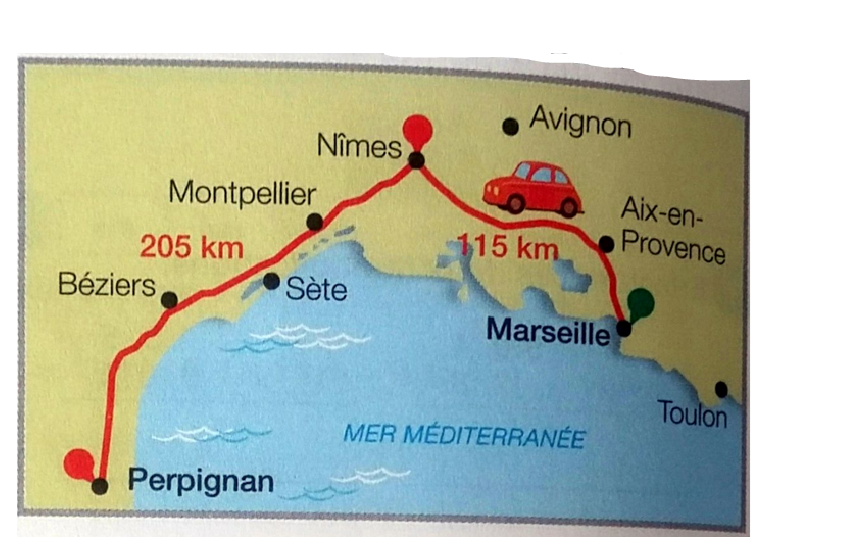
\includegraphics[scale=0.5]{pbmul5.eps} \\

Calculs en ligne : \\
\reponse[2]\\


Phrase réponse :\\
\reponse[1]\\

\end{document}
